\chapter[Apresentação do produto]{Apresentação do produto}
\section{Visão Geral}
Embora a apresentação do Agromart para uma CSA real não tenha sido um objetivo principal deste trabalho, tivemos a oportunidade de apresentá-lo à CSA da Florestta no dia 05/09/2024, na sede do Instituto Florestta em Taguatinga-DF, com a presença do professor e coorientador, Rudi Henri van Els. Após a apresentação, a atmosfera foi bastante positiva, e concluímos que o Agromart já possui as funcionalidades principais para ser utilizado por agricultores individuais. No entanto, constatou-se que o Agromart ainda não atingiu o nível de maturidade necessário para ser implementado em uma CSA real, com alguns pontos importantes levantados pela CSA da Florestta como essenciais para sua implantação.

\begin{figure}[h]
	\centering
	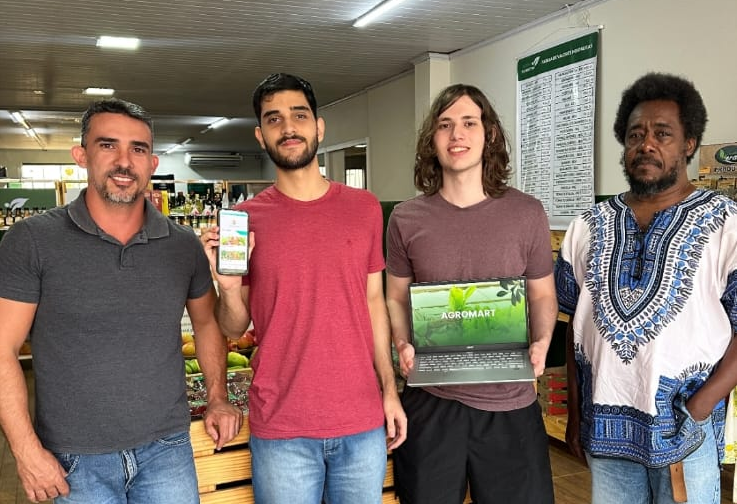
\includegraphics[keepaspectratio=true,scale=0.4]{figuras/apresentacao.png}
	\caption{Foto na sede da CSA da Florestta após a apresentação}
	\label{erro-ts-2}
\end{figure}

\section{Melhorias identificadas pela CSA da Florestta}
Essa seção tem como objetivo apresentar os pontos de melhoria destacados pelo administrador da CSA da Florestta para que o sistema do Agromart possa atender às necessidades de uma CSA real. Foram esses:

\begin{itemize}
    \item \textbf{Substituir o termo loja por pontos de convivência}: Dentro do contexto de uma CSA, os espaços em que o agricultor e o co-agricultor interagem são chamados de pontos de convivência ou pontos de coleta, o termo loja é evitado nesse contexto para evitar um entendimento equivocado de como uma CSA funciona.
    \item \textbf{Vincular os produtos à CSA}: Atualmente os planos e produtos estão sendo cadastrados dentro uma loja (ponto de convivência), no entanto, conversando com o administrador da CSA da Florestta, foi observado por ele que os planos e produtos devem estar vinculados à CSA, sendo cada ponto de convivência apenas o local onde o co-agricultor vai escolher receber os produtos.
    \item \textbf{Lembretes do recebimento das cestas}: Para o administrador da CSA, outro ponto muito importante que poderia ser incorporado ao Agromart, seria a funcionalidade de lembrete para o dia de entrega das cestas, que poderia ser tanto por meio de uma notificação no aplicativo quanto por uma mensagem no WhatsApp do co-agricultor.
    \item \textbf{Escolha do tipo de entrega}: No momento da finalização de um pedido, adicionar a funcionalidade de escolha do tipo de entrega, onde o co-agricultor informa se deseja realizar a retirada do produto ou recebê-lo em sua casa.
    \item \textbf{Flexibilizar periodicidade dos planos}: Atualmente os planos cadastrados no Agromart são sempre semanais, para atender as demandas de uma CSA real, é necessário possibilitar que a adesão aos planos tenha opções de diferentes periodicidades, como, por exemplo, o recebimento de cestas quinzenais.
\end{itemize}

Essas melhorias foram recebidas como sugestões importantes que podem guiar o desenvolvimento futuro do Agromart.